\section{Diffusive processes}\label{sec:diffusive_processes}
In formalising empirical observations of human gaze and neural activity into a mathematical model, this thesis relies on the framework of non-equilibrium statistical mechanics and stochastic calculus. When a system is driven by a massive number of microscopic interactions—such as the complex interconnected firing of a neural population—modelling the exact deterministic dynamics becomes intractable. Instead, statistical physics provides the tools to coarse-grain these high-dimensional systems into low-dimensional stochastic differential equations. This section establishes the mathematical progression necessary to model scale-free visual inference. We first review the classical paradigm of normal diffusion and Brownian motion (\cref{sec:brownian_motion}), which serves as the foundational model for standard diffusive physical systems. We then examine how systems of interest frequently violate the classical assumptions of normal diffusion and Brownian motion, leading to an understanding of the presence and role of anomalous diffusion in many complex dynamical systems (\cref{subsec:anom_diff}). Finally, we introduce Lévy stable motion (\cref{subsec:levy_motion}), a class of superdiffusive fractional stochastic processes that mathematically capture the heavy-tailed, intermittent dynamics characteristic of optimal visual search and neural activity.
\subsection{Brownian motion and normal diffusion}\label{subsec:brownian_motion}
Statistical modelling has been fundamental in understanding complex dynamical systems: separating the dynamics of macroscopic observables into deterministic terms and stochastic terms reduces chaotic high-dimensional systems to a small number of variables of interest \cite{hassler_stochastic_2016, cunchala2024basicoverviewvariousstochastic}. Stochastic processes are often the most natural, tractable, and accurate modelling tools when examining high-dimensional chaotic systems across physics, economics, geology, climate science, machine learning, and neuroscience \cite{[CITE]}. The universality of these stochastic models is understood to be an implication of the central limit theorem: the distribution of the summed effect of a large number of identical and independently distributed (i.i.d) random variables of finite mean and variance will approach a Gaussian \cite{ulyanov2024classical, heyde1978central, gnedenko1954limit}. The technique of treating a large number of independent coupled deterministic variables as a single stochastic variable turns out to be generalisable to a wide class of problems involving coupled, non-stationary, or diverging-variance processes which are out of equilibrium, such as in the case of neuronal spiking patterns \cite{18k5-pwl1, La_Camera_2022_meanfieldneuron}. The most ubiquitous stochastic process is central to statistical physics: the Brownian motion $W_t$, equivalently called the Wiener process, which consists of stationary and independent Gaussian increments across all non-overlapping time intervals. The Brownian motion is a very simple and analytically robust model of the coarse-grained effect of a high dimensional system of contributions which are flattened to a small number of observable dimensions. A Brownian motion is defined only by its timescale, with a variance over trajectories after time $t$ of $t$ itself. Realisations of Brownian motion yield time series' which are almost surely continuous but nowhere differentiable. Classical examples of processes modelled by the Brownian motion are: the movement of a macroscopic particle in a non-turbulent fluid \cite{hassler_stochastic_2016}, the gravitational influence of an orbiting collection of stars on supermassive black holes \cite{Chandrasekhar1943, Merritt2007a}, and (arguably) the movement of low-volatility stock prices \cite{cunchala2024basicoverviewvariousstochastic}. The generalisation of the Brownian motion for heavy-tailed i.i.d variables is a Lévy flight, and is described in detail in \cref{subsec:levy_motion}, and \cref{fig:brownian_vs_levy} compares the two processes.

To include random variables such as Brownian motion in dynamical systems, physicists and mathematicians have developed the tools of stochastic calculus. Brownian motion of a variable $\textbf{x}_t$ through time $t$ about a potential landscape $V(\textbf{x})$ can be described in terms of the first order Langevin equation:
\begin{equation}\label{eq:langevin}
    d\textbf{x}_t = -\gamma \nabla V(\textbf{x}_t) dt + \sqrt{2 \gamma} dW_t 
\end{equation}
where the constant $\gamma$ describes the noise strength of the Brownian motion \cite{smoluchowski1906zur, langevin1908theorie, uhlenbeck1930theory, kramers1940brownian} and $dW_t$ is a Brownian motion. Although the dynamics of $\textbf{x}_t$ is described stochastically, the dynamics of the corresponding probability distribution $P(\textbf{x},t)$ is deterministic and can be described exactly. Such an equation of motion of $P(\textbf{x},t)$ under any stochastic dynamics defining $\textbf{x}_t$ is called the Fokker-Planck equation \cite{boffi_probability_2023, jordan_variational_1998, wang1945theory, kolmogoroff1931analytischen, planck1917ueber, fokker1914mittlere}. In the case of \cref{eq:langevin}, the Fokker-Planck equation is \cite{jordan_variational_1998, boffi_probability_2023, planck1917ueber}
\begin{equation}\label{eq:overdamped-fokkerplanck}
    \partial_t P(\textbf{x},t) = \frac{\gamma}{2} \nabla \cdot \left( P(\textbf{x},t) \nabla V(\textbf{x}) + \nabla P(\textbf{x},t) \right)
\end{equation}
whose unique stationary distribution is the Boltzmann-Gibbs distribution
\begin{equation}\label{eq:boltzmann-gibbs}
    \pi(\textbf{x}) \propto \exp[-V(\textbf{x})]
\end{equation}
which yields the important relationship, where a 
Langevin potential can be constructed from a normalised target density via $V(\textbf{x}) = -\ln \pi(\textbf{x})$, which we will make use of in this thesis in constructing saliency maps from empirical data where only the likelihood of fixations $\pi(\textbf{x}))$ is given. %Importantly, the dynamical system defined by \cref{eq:langevin} is ergodic, and thus under \cref{eq:overdamped-fokkerplanck}, any initial distribution will converge to $\pi(\textbf{x})$. 
Importantly, the Langevin system Fokker-Planck equation \ref{eq:overdamped-fokkerplanck} will describe the diffusion of a sharply peaked initial distribution as it widens, and the statistics of this diffusion from a sharp initial condition define normal diffusion as follows. The solution to the Fokker-Planck equation from an exact initial condition $P(\textbf{x},0) = \delta^n(\textbf{x}-\textbf{x}_0)$ is dominated over short times by the $\nabla P$ term as $\nabla P \gg P \nabla V$, reducing the Fokker-Planck equation to the heat equation $\partial_t P = \frac{\gamma}{2}\nabla^2 P$. As such, the leading-order short-time solution is that of such a heat equation
\begin{equation}\label{eq:normal_diffusion}
    P(\textbf{x}, \Delta t) \propto \exp \left[ -\frac{\|\textbf{x} - \textbf{x}_0 \|^2}{2(\gamma \Delta t)}\right] \implies \text{Var}[\textbf{x}(\Delta t)] = \gamma \Delta t
\end{equation}
which demonstrates the interesting behaviour which defines normal diffusion: the short-time scaling of variance in position will be linear, as $\text{Var}[\textbf{x}_{\Delta t}] = \gamma \Delta t$. Thus $\gamma$ is often called the timescale of the Brownian motion, as it defines the rate of linear diffusion of variance with time. This linear scaling of the variance of trajectories with time defines normal diffusion \cite{klafter_anomalous_2005, vilk_strong_2025, sposini_towards_2022, oliveira_anomalous_2019}, and understanding those systems whose random motion does not reproduce such normal diffusion is crucial in understanding complex dynamical diffusion.
% The Fokker-Planck equation for the standard Brownian-Langevin system is a diffusion PDE equivalent to the heat equation with a gradient term, a correspondence well-understood before the development of stochastic calculus. The diffusion arising from such small uncorrelated perturbations of a dynamical system leads to the statistical properties which first drove the study of statistical physics, such as normal diffusion and the universality of Brownian motion, which we follow in \cref{subsec:anom_diff} and \cref{subsec:levy_motion} respectively, however the neural system described in this thesis diverges strongly from the Brownian paradigm, requiring an understanding of fractional processes.

% \subsubsection{Further stochastic models}
% Only recently have the universality of stochastic processes asides from the Brownian motion been well-studied. Of interest to this thesis is the case where microscopic perturbations become correlated and yield heavy-tailed statistics. Correlated steps, long-time memory effects, and chaotic microscopic dynamics can result in a stochastic process which does not limit to a Brownian motion \cite{Brevitt2025, Klages2013}. Of interest to us is the fractional \textit{Lévy flight}, a process driven by scale-free noise which span across many orders of magnitude. For instance, a spiking neural network at with diverging activity correlation length, where the centre of mass of neural firing is then subject to large jump discontinuities \cite{La_Camera_2022_meanfieldneuron, qi_fractional_2022, qi_fractional_2022}. Such large jumps in time series' are modelled with to Lévy stable noise, where the increments are drawn independently from a heavy-tailed distribution. This section describes the analytics, stability, and behaviour of such Lévy processes for our current study, and how their diffusive properties differ from the behaviour of Brownian motion.

\subsection{Anomalous diffusion}\label{subsec:anom_diff}
The universality of normal diffusion in systems which are driven by Brownian motion as above has been studied closely, most influentially as in the movement of particles in a fluid \cite{Einstein1905, klafter_anomalous_2005, metzler_anomalous_2014, Merritt2007a}. These dynamics inform the definition of normal diffusion through this variance scaling with time, rigorously calculated as the mean squared displacement (MSD) $\langle \|\Delta \textbf{x} (\Delta t) \|^2 \rangle \propto 
\Delta t$. To study the universality of such normally diffusive processes, the continuous time random walk (CTRW) model was developed, in which a trajectory has subsequent step sizes and durations drawn from finite variance distributions. Such models will universally reproduce this normal diffusive scaling property of $\langle \| \Delta \textbf{x} (t) \| \rangle \propto t$, and as a result of the central limit theorem, will approach Brownian motion. However, increasingly interesting physical systems have been found which diffuse nonlinearly in time, a situation known as anomalous diffusion, with an MSD scaling as:
\begin{equation}
    \langle \| \Delta \textbf{x} (\Delta t) \|^{2} \rangle \propto \Delta t^{\lambda_2}, \ \ \lambda_2 \neq 1
\end{equation}
Such anomalous diffusion yields two cases, subdiffusion $0 < \lambda_2 < 1$ where diffusion scales slower than normal, and superdiffusion $1 < \lambda_2 < 2$ where diffusion scales faster than normal. The case of $\lambda_2 = 2$ is known as ballistic diffusion, as it is found in the deterministic case of constant velocity $x = vt$. An important phenomenon often found in diffusive processes is fractal self-similarity. A Brownian motion is self-similar across all scales, and is nowhere smooth,  and in physical systems demonstrating anomalous diffusion, self-similarity resulting from criticality is often reported. Later in \cref{subsec:levy_motion}, we will find that it is advantageous in the study of anomalous superdiffusion to capture this multi-scale diffusive self-similarity through an extension of the $\lambda_2$ scaling of MSD to a spectrum of absolute moments $\lambda(q)$ which describes the diffusive self-similarity which unifies across many scales of study. A comparison of Brownian motion and Lévy motion which displays their self-similar properties and diffusive scaling through the mean absolute displacement $\langle \|\Delta \textbf{x}\| \rangle \propto \Delta t^{\lambda_1}$ is shown in \cref{fig:brownian_vs_levy}.

Anomalous subdiffusion has been shown to result from heavy-tailed wait-times between interactions \cite{klafter_anomalous_2005}, such as in trapped fluid flow \cite{Kirchner2000-kf}, controlled diffusion through cell membranes \cite{klafter_anomalous_2005}, and protein mixing \cite{Kou2004-kz}. 
\subsubsection*{Anomalous superdiffusion}\label{subsubsec:anomalous_superdiffusion}
Of great importance in studying the dynamcs of visual search, superdiffusion has been studied in the contexts of complex exploratory biological systems. We model the efficient exploration of gaze dynamics through Lévy superdiffusion, which is the standard dynamical model of superdiffusion in physics and is presented in detail in \cref{subsec:levy_motion}. Such Lévy superdiffusion has a strong link to the problem of designing a strategic search for scarce resources. However the true computational benefit of superdiffusion has become a subject of debate in the literature. On one side, the Lévy foraging hypothesis posits that the standard superdiffusive CTRW, the Lévy walk, is an optimal strategy when searching for sparse and randomly distributed resources. On the other, researchers have proposed that such a model is biologically unrealistic and a result of artificial modelling conditions. 

The finding that Lévy superdiffusion is optimal in random search was first reported in a letter to the journal Nature in 1999 by \textcite{viswanathan_optimizing_1999}. In the original paper proposing the Lévy foraging hypothesis a Lévy walk with superdiffusion $\langle x(t) ^2 \rangle \propto \frac{t^2}{\ln(t)}$ on the transition to ballistic diffusion was found to be optimal in a search for sparse resources \cite{viswanathan_optimizing_1999}. Recently, physicists and biologists have questioned if this result is imposed by an unrealistic modelled task, an argument described most strongly just this year by \textcite{pyke_levy_2026}, as well as in general analyses of superdiffusion in \cite{reynolds_liberating_2015, benhamou_ultimate_2015, pyke_understanding_2015}. However, despite such disagreement, the optimality of the superdiffusive Lévy walk has been reproduced in diverse functional search models \cite{humphries_optimal_2014, campeau_evolutionary_2022, sims_optimal_2019}, in a population of diverse searching agents with a range of superdiffusive exponents $\lambda_2$ \cite{clementi_search_2021} as well as in a large study against several different search conditions \cite{humphries_optimal_2014}, and have been reported in the empirical search paths of biological organisms from the flights of drosophila flies \cite{sims_optimal_2019, reynolds_free-flight_2007}, albatross' searches \cite{focardi_levy_2014, humphries_new_2013}, and strongly across many marine predators \cite{sims_scaling_2008, humphries_environmental_2010}. 

The result of these analyses yields a complex understanding of Lévy superdiffusion, advantages of Lévy walks have been shown to be model-dependent, with the optimal performance of Lévy walks requiring biologically inaccurate depictions of search paths \cite{pyke_levy_2026, gautestad_levy_2013, pyke_understanding_2015}. These arguments marks a split in the treatment of Lévy walks, with groups studying them as informative baseline functional models of abstract search \cite{viswanathan_optimizing_1999, gautestad_levy_2013, humphries_optimal_2014, clementi_search_2021}, and others led by Graham Pyke presenting this as a misrepresentation of true intelligent organisms \cite{pyke_levy_2026, pyke_understanding_2015, benhamou_ultimate_2015}. This thesis provides a biologically realistic and well-motivated superdiffusive search for research into a case for optimal Lévy motion. See \textcite{reynolds_liberating_2015} for an in-depth discussion of a richer view of biological Lévy superdiffusion.
\subsection{Lévy motion}\label{subsec:levy_motion}
\begin{figure}[h!]
	\centering
	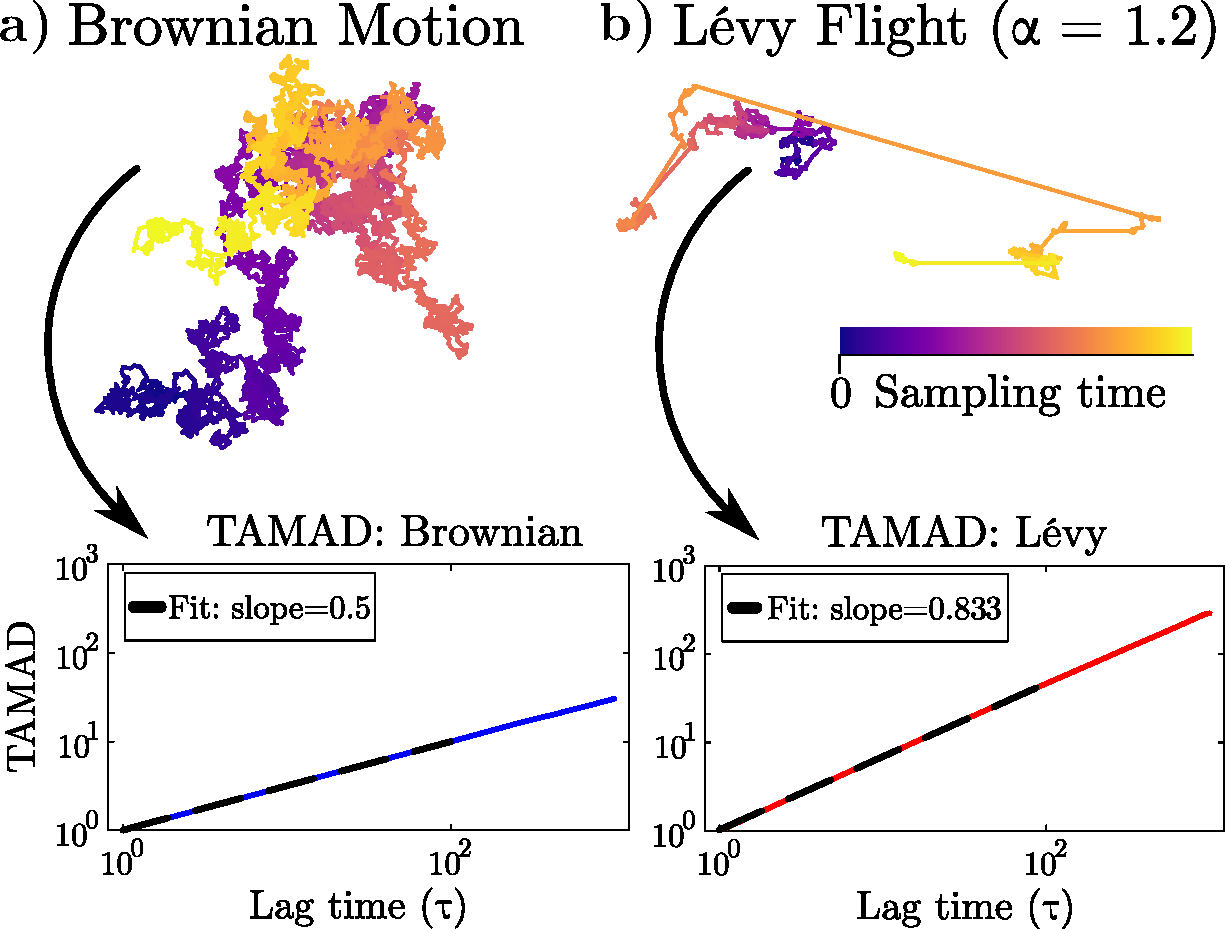
\includegraphics[width=0.8\linewidth]{figures/BvL.pdf}
	\caption{\textbf{Schematic representations of stochastic motion and their respective diffusion.} \textbf{a)} Schematic representation of a 2D Brownian motion, along with its time-averaged mean absolute displacement (TAMAD), which is the $q=1$ mean fractional displacement as in \cref{eq:MFD}. Normal diffusion is here present as a power law slope of exponent $1/2$, giving diffusive exponent $\beta=1$ as defined in \cref{eq:MFD}. \textbf{b)} Schematic of a superdiffusive 2D Lévy flight with characteristic exponent of $\alpha=1.2$, and a MAD slope of $0.833$ corresponding to the theoretical superdiffusive coefficient $\beta= 2/\alpha = 5/3$.}
	\label{fig:brownian_vs_levy}
\end{figure}
To mathematically capture the intermittent, scale-free nature of visual search, we turn to the Lévy flight: a superdiffusive stochastic process that permits close analysis, due to it's very foundational mathematical definition. Here, the Lévy flight $L_t^{\alpha}$ is a stochastic process defined through it's increments being drawn from a heavy tailed symmetric $\alpha$-stable distribution (a $\mathcal{S}\alpha\mathcal{S}$ distribution), where $\alpha$ is called the characteristic exponent and relates to the exponent of the distributions powerlaw tails. $\mathcal{S}\alpha\mathcal{S}$ distributions describe the limit of summation of i.i.d infinite-variance variables, as a result of the generalised central limit theorem, making them ideal to describe a universality class of superdiffusive processes. The $\alpha$ value defining a particular $\mathcal{S}\alpha\mathcal{S}$ distribution is a result of the asymptotic power-law tail of the density function, with the probability density function following $p(x) \propto |x|^{-1-\alpha}$. As a result, the Lévy flight $L_t^{\alpha}$ after time $t$ is defined by its fractional scaling properties and alpha-stable statistics
\begin{equation} \label{eq:levy_noise}
	L_t \stackrel{d}{=} t^{1/\alpha} L_1, \ \ L_1 \sim \mathcal{S}\alpha\mathcal{S}
\end{equation}
where $\stackrel{d}{=}$ denotes equal in distribution. In the limit $\alpha \rightarrow 2$, the Lévy flight reduces to a scaled Brownian Motion $L_t^{\alpha \rightarrow 2} = \frac{1}{\sqrt{2}}W_t$. If $1 < \alpha < 2$ the variance of $L_t^{\alpha}$ diverges and has mean 0, whereas if $0 < \alpha \leq 1$, then both the variance and mean diverge. In analysing the distribution of a Lévy flight, one must generalise the standard Langevin Fokker-Planck equation (\ref{eq:overdamped-fokkerplanck}) to the Lévy motion using fractional calculus to capture the nonlocal transport of the particle. The details of such an analysis are beyond this thesis, however the fractional Fokker-Planck equation is the tool used to understand the superdiffusion, nonlocality, and scale-free behaviour of trajectories of Lévy flights (see the appendices to \cite{qi_fractional_2022}). Many of the simple analytic properties of the Brownian motion are no longer true of a Lévy flight. Notably, since these flights have infinite variance in steps sizes, the mean squared displacement diverges. Thus their superdiffusion is better measured using an extension of MSD to fractional absolute displacements, through the definition of the moment spectrum function $\lambda(q)$ as in \cite{vilk_strong_2025}:
\begin{equation}\label{eq:MFD}
	\langle \| \Delta \textbf{x}(t) \| ^ q \rangle \propto t^{\lambda(q)}, \ \ q > 0
\end{equation}
where $q$ is the order of the fractional absolute displacement, and the power law slope will converge for an $\alpha$-Lévy flight to $\lambda(q) = q/\alpha$ when $q < \alpha$. As such, for Lévy flights with exponents $\alpha > 1$ superdiffusion is well-characterised by the mean absolute displacement, where $q=1$ in \cref{eq:MFD}.

Importantly, trajectories of a Lévy flight are no longer continuous. Instead, such trajectories are called \textit{càdlàg} (continue à droite, limite à gauche) with respect to time, which describes functions which are right continuous with well-defined left limits \cite{van_den_Bosch}. Thus, we say that since all such trajectories produced from a Lévy flight are càdlàg, the Lévy flight itself is called a càdlàg process. Càdlàg processes have been widely studied in the context of mathematics, economics, and physics, and their properties are well understood \cite{soulier2022-ge, Borkar1995}. It has been shown that Lévy flights are semimartingales, and are well interpreted in integration \cite{van_den_Bosch}. Importantly, it follows from the Lévy-Itô decomposition theorem that a Lévy flight can be decomposed as the sum of two processes \cite{Kyprianou2014}:
\begin{enumerate}
	\item A compound Poisson process of large jumps with $\| \Delta \textbf{x} \| > 1$. Such jumps are exponentially distributed in time, and there are almost surely a finite number in any finite time period.
	\item A square-integrable martingale (mean 0) jump process with $\| \Delta \textbf{x} \| < 1$. This process is then finite-variance, and as such is subject to the central limit theorem, meaning that under temporal coarse graining it approaches a Brownian motion.
\end{enumerate}
This division is useful in analysing the process in the context of nonlocal stochastic exploration in Lévy flights, which is modelled by the compound Poisson process of large jumps $|\Delta \textbf{x}| > 1$, and the local exploitation dynamics modelled by the square-integrable martingale of small jumps $|\Delta \textbf{x}| < 1$. In the context of visual searching, such a division naturally inspires the division between large jumps of attention, and periods of prolonged attention. As such, we are interested in why such superdiffusive scale-free dynamics may have a powerful in computational advantage in exploring an abstract unknown landscape.

%\subsection{Nested oscillations}